% !TeX spellcheck = en_US
% !TEX root = ../thesis-example.tex
%
\chapter{Evaluation \& Conclusion}

This mixed reality pipeline is capable of not only integrating the VR actor 
into the environment, but enhancing the motion video feed with additional 
parameters gathered from the engine, like lightning informations and stencils 
for the camera image (fig. \ref{fig:eval:results}). With that it is now 
possible to have an immersive view into a virtual environment and recording 
footage with a broad amount of hardware. Following section with empathize some 
considerations and possible variations with this system.

\begin{figure}[htbp]
	\caption{Results}
	\label{fig:eval:results}
	\centering
	\begin{subfigure}[t]{\textwidth}
		\centering
		\includegraphics[width=\textwidth]{gfx/results/pano.png}
		\caption{Current studio setup --- \circled{a} green screen; 
			\circled{b} Panasonic Lumix GH2; \circled{c} PC Workstation}
	\end{subfigure}
	\begin{subfigure}[t]{.49\textwidth}
		\centering
		\includegraphics[width=\textwidth]{gfx/results/camera.png}
		\caption{System components --- \circled{a} Panasonic Lumix GH2; 
			\circled{b} Controller Tripod Mount; \circled{c} INOGENI 4KUSB3 
			HMDI 
			converter; \circled{d} HTC Vive Controller; \circled{e} HTC Vive 
			HMD}
	\end{subfigure}
	\hfill
	\begin{subfigure}[t]{.49\textwidth}
		\centering
		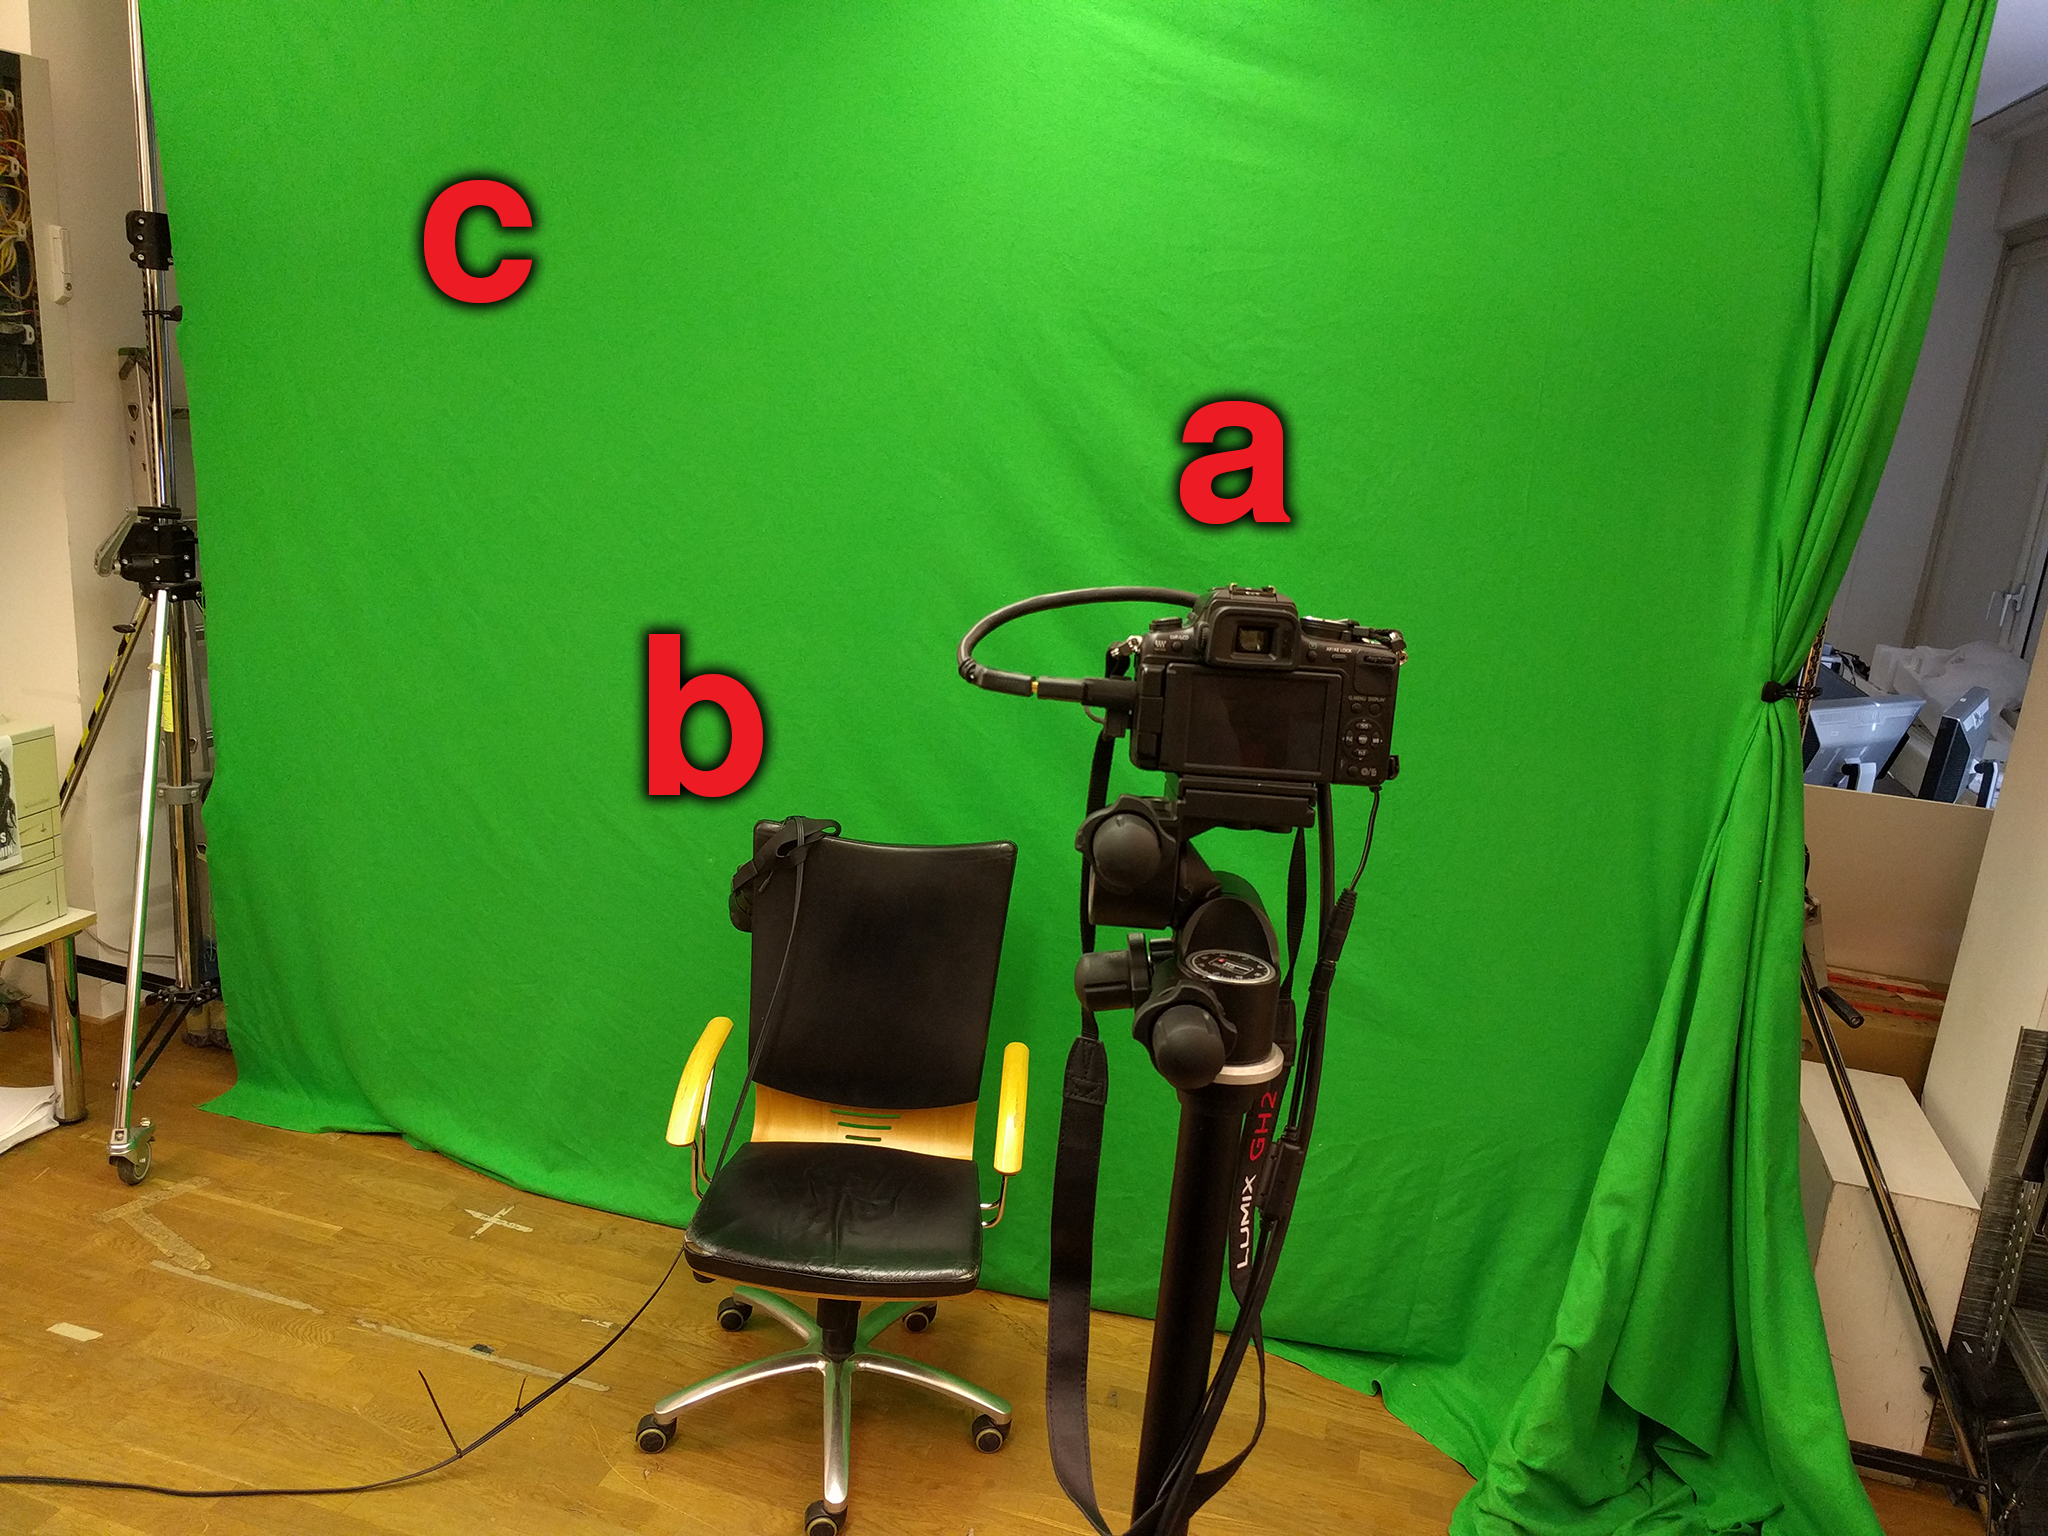
\includegraphics[width=\textwidth]{gfx/results/set.png}
		\caption{\circled{a} Panasonic Lumix GH2; \circled{b} HTC Vive HMD; 
			\circled{c} green screen}
	\end{subfigure}
	\begin{subfigure}[t]{.49\textwidth}
		\centering
		\includegraphics[width=\textwidth]{gfx/results/pc.png}
		\caption{PC Workstation}
	\end{subfigure}
	\hfill
	\begin{subfigure}[t]{.49\textwidth}
		\centering
		\includegraphics[width=\textwidth]{gfx/results/mr-action_new.png}
		\caption{final Mixed Reality composition}
	\end{subfigure}
	\begin{subfigure}[t]{.49\textwidth}
		\centering
		\includegraphics[width=\textwidth]{gfx/results/self-illu.png}
		\caption{Self-Illumination from virtual light casted on real world 
			camera image}
	\end{subfigure}
	\hfill
	\begin{subfigure}[t]{.49\textwidth}
		\centering
		\includegraphics[width=\textwidth]{gfx/results/mr-action_old.png}
		\caption{another, earlier Mixed Reality composition}
	\end{subfigure}
\end{figure}

\section{Hardware Setup Variations}
\label{sec:eval:hardware}

Due to the nature of the setup and fine-tweaking options inside the engine, 
this approach discussed in the previous section can have a wide variety of 
operational setups. By lose coupling of these hardware factors there are only a 
few limitations that can either be solved by better, future hardware or a 
different approach that are outside of the scope.

An integral part of this setup is the motion tracking solution: it is possible 
to hook up an Oculus Rift\footnote{with its room-scale setup} instead of the 
HTC Vive and set one controller as camera-attachment point. For that there 
would be another 3D print needed to attach the controller to a camera solution. 
\newline
Other third market VR-HMDs usually follow the Vive's specifications closely and 
integrate natively with SteamVR, thus no modification on the original 
instalment has to be done.
\newline
Through Virtual Reality Peripheral Network or OpenVR simliar solutions can be 
developed, since none of the software explicitly depends on SteamVR features 
and allow a wide variety of systems and sensors.

The video capturing side can be varied greatly too, since the software only 
requires for webcam-compatible devices, it would be possible to remove 
the Inogeni encoder and replace it with cheap and simple webcams. Similarly, 
can a camera be replaced along with other recording solutions, as long as it 
outputs an HDMI (or HDMI-convertible) video stream. This allows recording to be 
as complex as needed but in general a DSLR camera will suffice.

\section{3D Environment and Composition Considerations}

While working with this pipeline, some problematic cases were discovered, which 
generally do not work well with mixed reality. Very cluttered environments can 
easily have obstructing meshes that clip --- partially or completely --- 
through the virtual camera frustum and obstruct 3D projection. Minimizing this 
issue can be done by either disallowing a user to move the SteamVR bounding box 
at all, only allow for certain teleporting positions or do permit 
teleportations altogether that potentially clip through the SteamVR bounding 
box.
\newline
A green screen is crucial for a live performance and recent papers focus only 
on increased accuracy with unacceptable computation times in this context. Due 
to the needs of a studio-like setup it is additional overhead for having a 
mobile, transportable experience. However the gains of Mixed Reality might be 
very well worth it. 
\newline
By placing a virtual monitor showing the final mixed reality composition it is 
possible to communicate and contextualize the real world actors performance 
back to himself, allowing him to have a third person perception of his actions.

\section{Performance Considerations}

Due to the nature of this rendering pipeline there is a significant performance 
overhead caused --- since multiple virtual cameras are capturing the scenery at 
a high frame rate --- and it is overall very taxing on the GPU. Each camera 
change causes, including the two VR projections, multiple context changes, 
which additionally slows down performance. The $\Delta E$ chroma keying 
operation runs twice per pixel through an if/else case which is 
likely\footnote{Unfortunately the Unity GPU profiler does not provide that 
data and external GPU debuggers seem to simply crash while attaching to Unitys 
rendering context} evaluated on both cases and later one of those is used, 
adding another layer of computation complexity on top. 
\newline
The pipeline is already built in such a way as to reduce the amount of cameras, 
but needs at least 4 virtual projections. Each feature --- except fore- and 
background  rendering --- can be disabled to ease the performance hit. With 
that in place it is possible to balance between accuracy and computation speed 
--- with further considerations by doing full mixed reality on mobile phones or 
different performing devices, a dynamic rendering pipeline could be created 
that manages composition modes on runtime. Further exploration could be done to 
include Valve's "The Lab Renderer" which also manages asset fidelity and 
rendering operations dynamically to hit an optimal frame rate. Future work 
could involve a reduced sampling rate on the chroma key operations for further 
performance improvement.
\newline
This pipeline is able to render about 120.000 triangles with pre-baked 
lightning and disabled post-fx on the set PC. This works well for small 
room-sized experiences but likely needs more performance improvement for 
more ambitious looking scenery.

Finally, since the full pipeline is rather complex, a good desktop PC will be 
needed. The CPU overhead is minimal but the graphical complexity is based on 
limitations of the GPU. With future iterations of this hardware it will be 
possible to create more complex scenery, output higher resolution video and 
better frame rates if the video capture device allows for it.
\newline
In theory, a low-poly environment could be render-able on mobile, combined with 
a low sample rate on the camera image, to produce a "window" into VR for 
multiple users at the same time, thus enabling an indefinite view into virtual 
reality. This would remove the MR-pipeline from an actor's system. Further work 
could tap into a Microsoft HoloLens solution, which could enable a direct 
contextualization of an actor into a VR scenery without a green screen at all. 
With fast approximate algorithms, like YCgCo-keying, this could produce a 
high-framerate transparent overlay, so that the virtual scene does not clip the 
actor.

\section{Edge Cases}

The proposed method has edge cases which could be further improved by other 
approaches in rendering or capturing actor video. These highlight issues 
observed with the rendering operations discussed in this thesis.

\subsection{Image Clipping --- Incorrect Z Calculation for Hands}

Due to the planar projection of the real world feed inside the engine, any 
Z-information of the actor is squashed to a fixed depth. This means that hands 
are on the same plane. In cases with high z-difference between actor and 
actor's hands, it is possible that hand motion look unnatural and does not seem 
like it is to be supposed --- in figure \ref{fig:edge:z-clipping} is an actor 
depicted, whose hands are clearly in front of a virtual cube. The produced 
mixed reality image shows his arms only behind the cube.

\begin{figure}[htb]
	\centering
	\includegraphics[width=\textwidth]{gfx/issues/z-clipping.png}
	\caption{The actors hands do not visibly reach through the blue cube and 
	the actor shears it because of the planar projection}
	\label{fig:edge:z-clipping}
\end{figure}

One solution for future research could be acquiring an actor's depth by either 
using Time of Flight cameras and using a resulting point cloud or by 
calculating each camera pixel's depth with a stereoscopic solution. Thus each 
pixel could have a quantifiable depth with additional calibration parameters 
from the virtual reality tracking solution.

\subsection{Matting Failures}

There are multiple problems with green screens, which are as old as green 
screens are used in video production. First and foremost is a partial 
transparent actor if his clothing consists of similarly green shaded material.
\newline
Additional green screen spill causes artifacts while pulling the matte which 
then clips the actor off (fig. \ref{fig:issue:blur}a). This can be mitigated 
by better production 
environments, i. e. with higher quality cloth and a generally well lit 
set\footnote{Appendix \ref{app:lightningsetup} features a basic schematic of a 
small green screen setup.}.
\newline
Sometimes, for example in low light environments or folded green screen 
material, the background covers a wide color range, thus calibrating a good 
green with a single color value is nearly impossible. This could be solved by 
smaller selection margins inside the shader while assigning an array of colors 
for the $\Delta E$ calculation. In turn, this would be even more taxing on the 
GPU, since the calculation has be done per selected color, multiplying the 
effort by the number of colors.
\newline
Lastly, real time chroma keying has problems with motion blur of the source 
video material --- causing background mixing and invalid matting (fig. 
\ref{fig:issue:blur}b). This is a complex problem that is far beyond the scope 
of this thesis. One of the best solutions is a color unmixing approach 
researched by Disney and "typically requires 10s for local color estimation 
(assuming 8 dominant colors), another second to propagate the local color model 
to the following frame, and approximately 3s for color unmixing." 
\cite{disney:unmixing:2017}

\begin{figure}
	\begin{subfigure}[t]{.45\textwidth}
		\centering
		\includegraphics[width=\textwidth]{gfx/issues/spill.png}
		\subcaption{Color spill from the green screen tints the clothing of the 
		VR actress, yielding incorrect chroma keying results}
	\end{subfigure}
	\begin{subfigure}[t]{.45\textwidth}
		\centering
		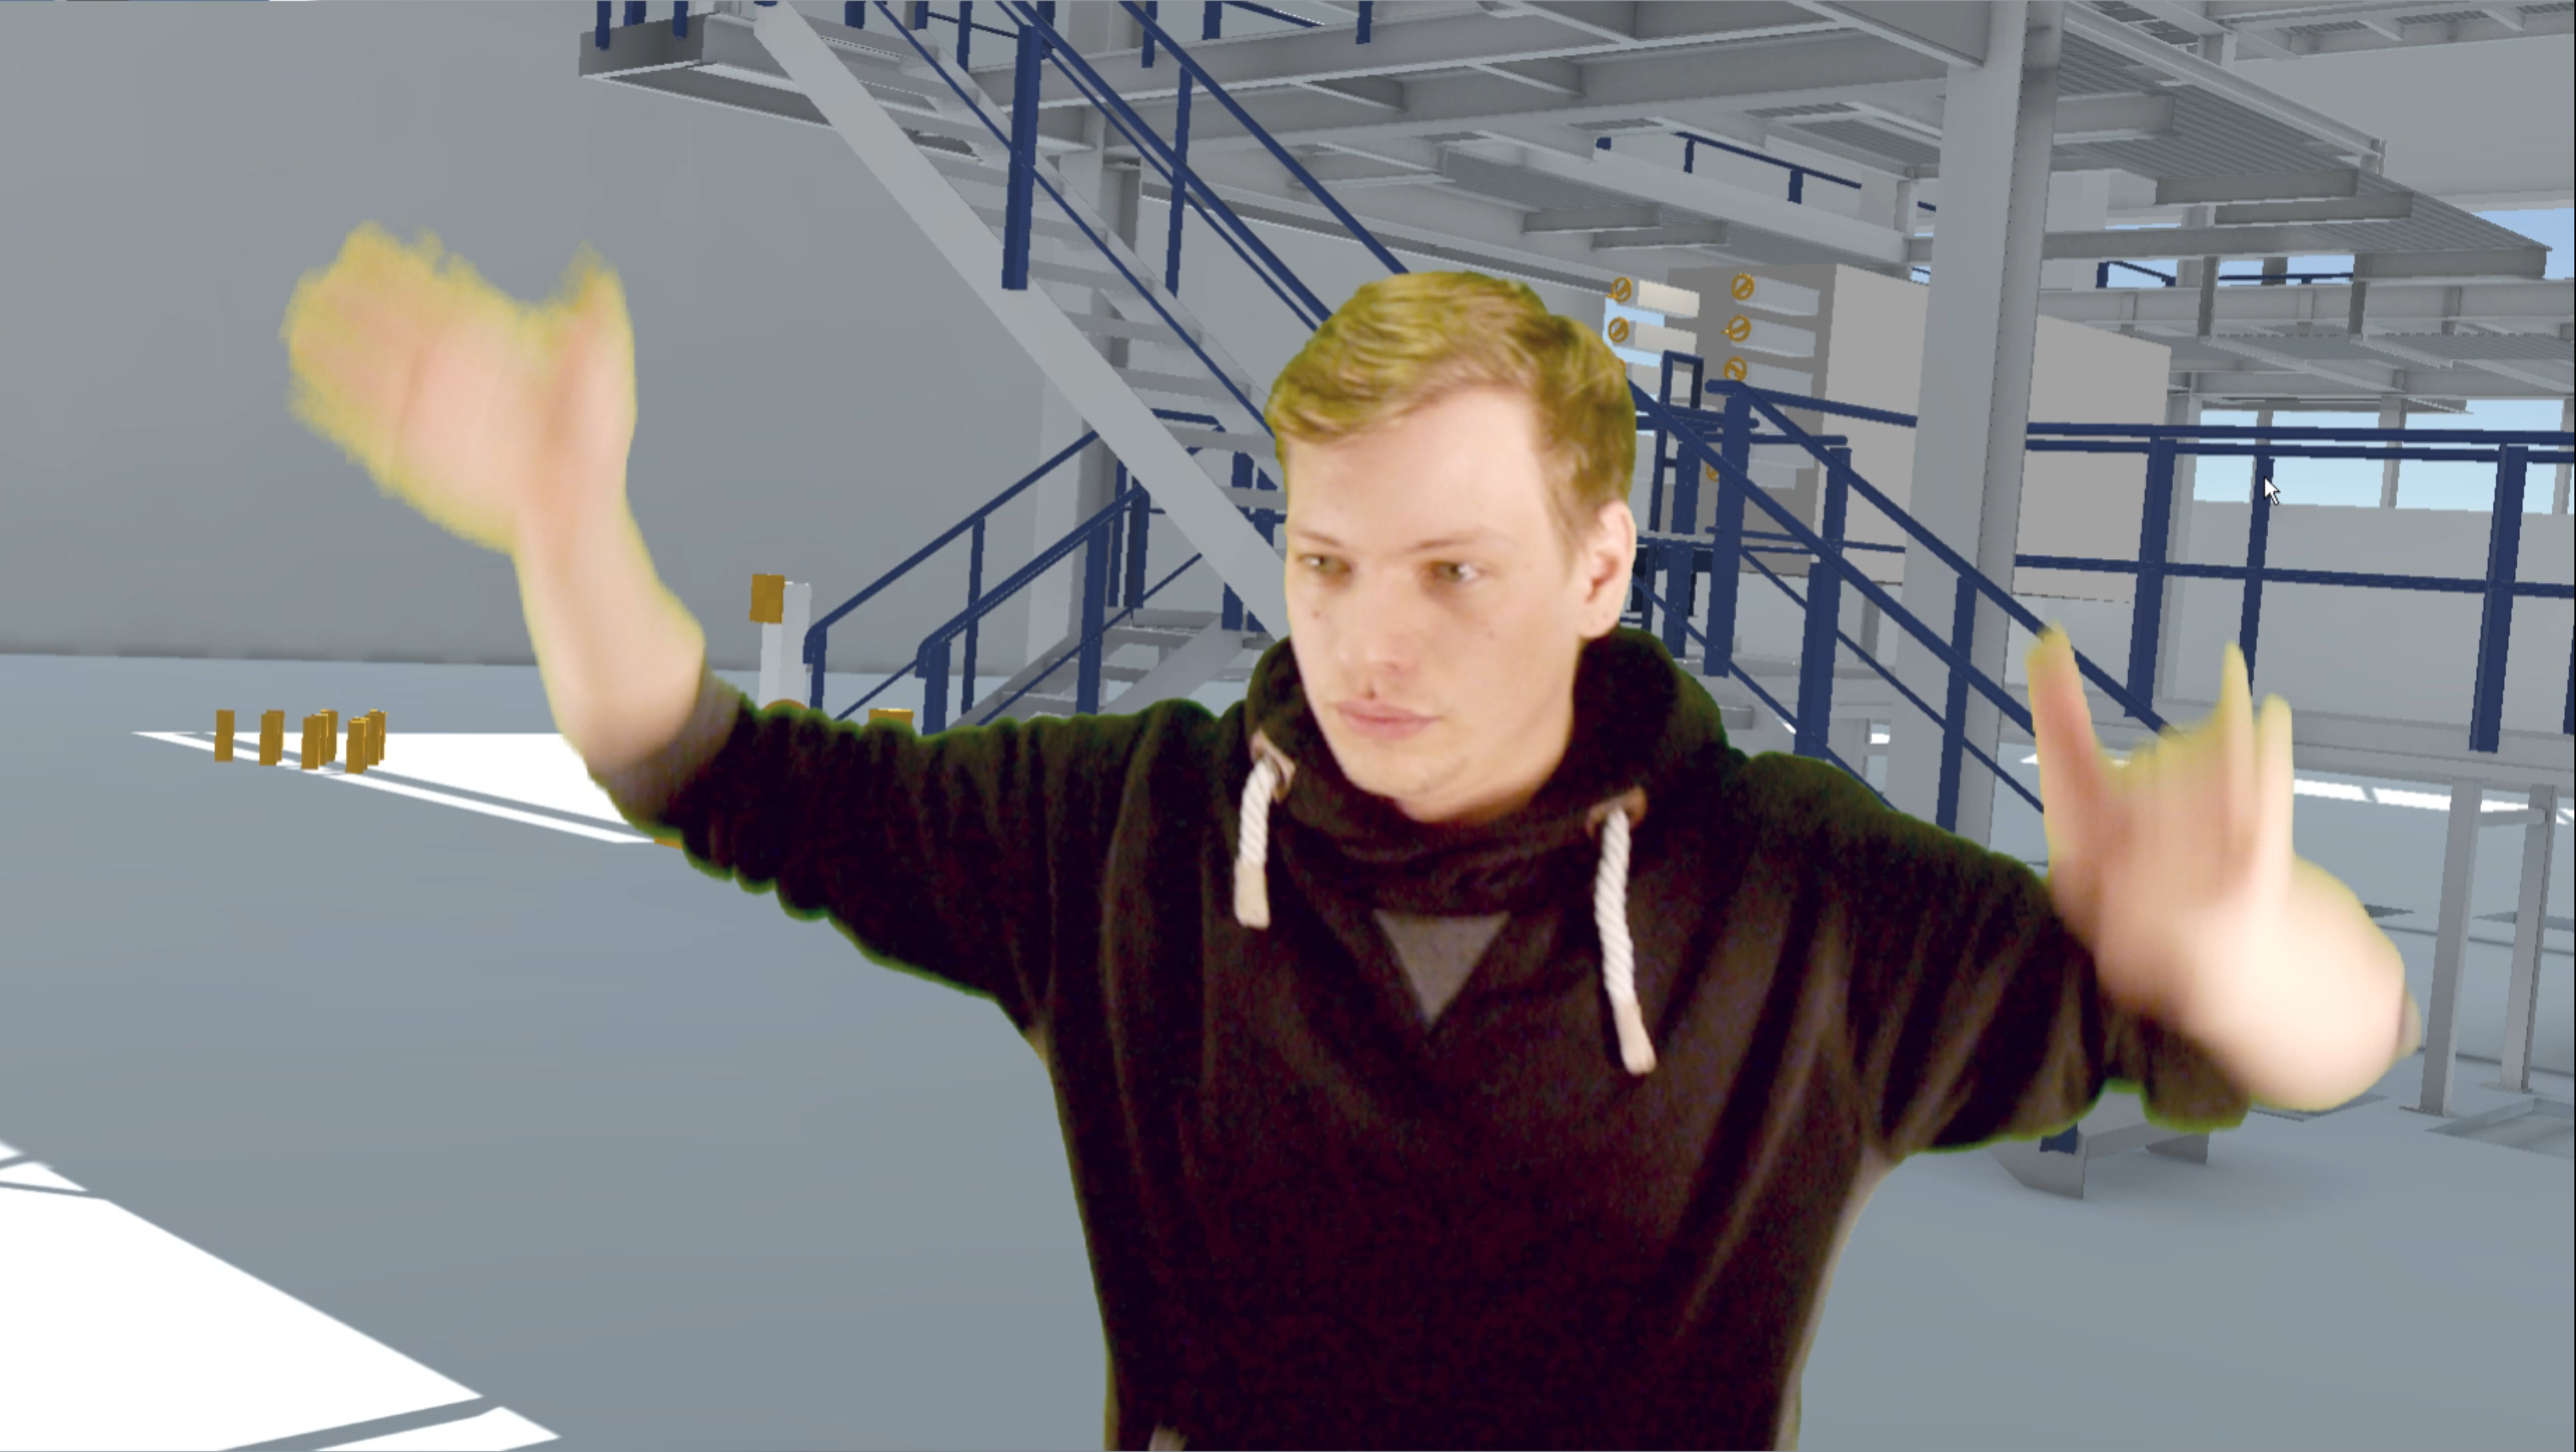
\includegraphics[width=\textwidth]{gfx/issues/blur.png}
		\subcaption{Due to motion blur in the source video material, it is 
		impossible for the software to determine between fore- and background}
	\end{subfigure}
	\caption{Examples of matting failures inside the software}
	\label{fig:issue:blur}
\end{figure}

\subsection{Calibration Problems}

The biggest margin of error is calibration of all projection parameters.
\newline
Beginning from field of view calculation, most DSLR cameras don't have 
specifications for their output feeds, where, for example, scaling factors 
could change the field of view angle. If these are not given or seem to be 
unfitting in production it is necessary to measure these parameters by hand, 
fixing the cameras position and calculating the spanning angle.

Another factor are offset-parameters between controllers and camera sensor, 
which have been minimized by the 3D printed attachment. However, minimal 
differences in this transformation matrix have tremendous impact on 
miscalculated projections, visible by wrongly placed objects and a disconnect 
between virtual interaction and actor.

Lastly, the most time spent after adding all mixed reality components to the 
scene is calibrating these parameters. There is a possible room of improvement 
by researching different calibration methods, since one controller can be 
guided by the user inside the frustum of the real world camera.